\documentclass{report}

\usepackage{graphicx}
\usepackage{algorithm}
\usepackage{array}
\usepackage{dsfont}
\usepackage{algpseudocode}
\usepackage{listings}
\usepackage{amsmath}
\usepackage{tikz}
\usepackage{pdfpages}
\usepackage{float}

\usetikzlibrary{automata, positioning, arrows}
\DeclareMathOperator{\rank}{rank}
\makeatletter
\newenvironment{sqcases}{%
  \matrix@check\sqcases\env@sqcases
}{%
  \endarray\right.%
}
\def\env@sqcases{%
  \let\@ifnextchar\new@ifnextchar
  \left\lbrack
  \def\arraystretch{1.2}%
  \array{@{}l@{\quad}l@{}}%
}
\makeatother

\usetikzlibrary{calc}


\input{/mnt/fa80f336-3342-4d78-8bfd-a43e434a2cda/Latex/preamble.tex}
\input{/mnt/fa80f336-3342-4d78-8bfd-a43e434a2cda/Latex/macros.tex}
\input{/mnt/fa80f336-3342-4d78-8bfd-a43e434a2cda/Latex/letterfonts.tex}

\title{\Huge{FU08 \-- Automata and Languages}\\Exercise 6}
\author{\huge{NGUYEN Tuan Dung}\\\huge{s1312004}}
\date{December 27, 2024}

\begin{document}

\maketitle

% Cau 1
\qs{Convert the folowing finite automata into equivalent regular expressions}{
$M=\left(Q, \sum, \delta, q_0, F\right)$ with\\
$ Q=\left\{q_0, q_1, q_2, q_3, q_4\right\} \\
  \sum=\{0,1\} \\
  F=\left\{q_4\right\}, \text { and } \delta \text { is defined by } $
  \begin{table}[H]
    \centering
    \begin{tabular}{|c|c|c|}
    \hline
    $\delta$ & 0    & 1    \\ \hline
    $q_0$                  & $q_1$ & $q_3$ \\ \hline
    $q_1$                  & $q_1$ & $q_4$ \\ \hline
    $q_2$                  & $q_2$ & $q_1$ \\ \hline
    $q_3$                  & $q_4$ & $q_3$ \\ \hline
    $q_4$                  & $q_2$ & $q_4$ \\ \hline
    \end{tabular}
\end{table}}

\sol{\newline
From the state transition table, we construct the DFA.\\

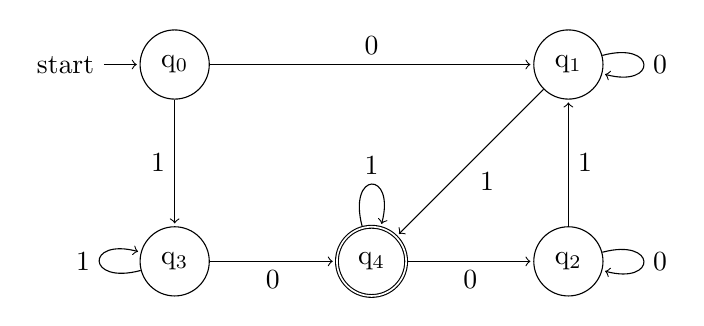
\begin{tikzpicture}[shorten >=1pt, node distance=2.5cm, on grid, auto][h]
  \node[state, initial] (q0) {$\mathrm{q}_{0}$};
  \node[state, draw=none] (a) [right=of q0] {};
  \node[state] (q1) [right=of a] {$\mathrm{q}_{1}$};
  \node[state] (q2) [below of=q1] {$\mathrm{q}_{2}$};
  \node[state] (q3) [below of=q0] {$\mathrm{q}_{3}$};
  \node[state, accepting] (q4) [right=of q3] {$\mathrm{q}_4$};

  \path[->]
    (q0) edge node {0} (q1)
        (q0) edge node[left] {1} (q3)
    (q1) edge [loop right] node {0} (q1)
        (q1) edge node {1} (q4)
    (q2) edge node[right] {1} (q1)
        (q2) edge [loop right] node {0} (q2)
    (q3) edge [loop left] node {1} (q3)
        (q3) edge node[below] {0} (q4)
    (q4) edge [loop above] node {1} (q4)
        (q4) edge node[below] {0} (q2);
\end{tikzpicture}
\\
\begin{minipage}[h]{0.48\textwidth}
\noindent $\bullet$ Step 1: Insert a new end state.\\
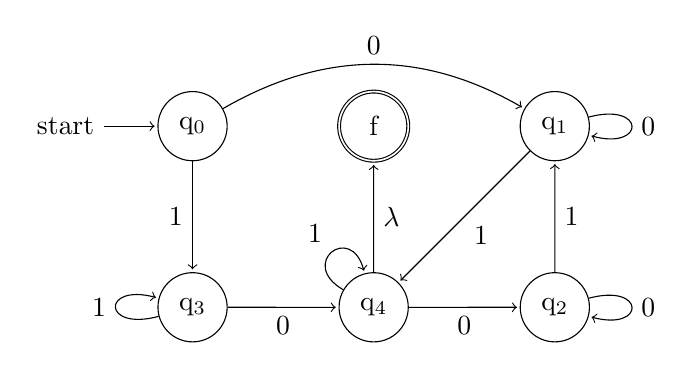
\begin{tikzpicture}[shorten >=1pt, scale=1.5, node distance=2.3cm, on grid, auto][h]
    \node[state, initial] (q0) {$\mathrm{q}_{0}$};
    \node[state, accepting] (a) [right=of q0] {f};
    \node[state] (q1) [right=of a] {$\mathrm{q}_{1}$};
    \node[state] (q2) [below of=q1] {$\mathrm{q}_{2}$};
    \node[state] (q3) [below of=q0] {$\mathrm{q}_{3}$};
    \node[state] (q4) [right=of q3] {$\mathrm{q}_4$};
  
    \path[->]
      (q0) edge[bend left] node {0} (q1)
          (q0) edge node[left] {1} (q3)
      (q1) edge [loop right] node {0} (q1)
          (q1) edge node {1} (q4)
      (q2) edge node[right] {1} (q1)
          (q2) edge [loop right] node {0} (q2)
      (q3) edge [loop left] node {1} (q3)
          (q3) edge node[below] {0} (q4)
      (q4) edge [loop, in=105, out=150, looseness=5] node {1} (q4)
          (q4) edge node[below] {0} (q2)
        (q4) edge node[right] {$\lambda$} (a);
  \end{tikzpicture}
\end{minipage}
\hfill
\begin{minipage}[h]{0.48\textwidth}
\noindent $\bullet$ Step 2: Rip $\mathrm{q}_3$.\\
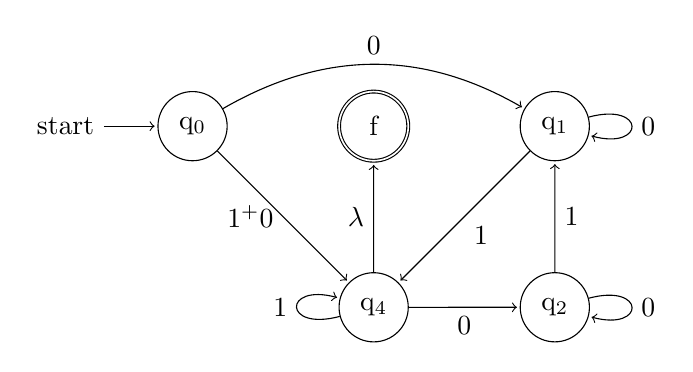
\begin{tikzpicture}[shorten >=1pt, scale=1.5, node distance=2.3cm, on grid, auto][h]
    \node[state, initial] (q0) {$\mathrm{q}_{0}$};
    \node[state, accepting] (a) [right=of q0] {f};
    \node[state] (q1) [right=of a] {$\mathrm{q}_{1}$};
    \node[state] (q2) [below of=q1] {$\mathrm{q}_{2}$};
    \node[state, draw=none] (q3) [below of=q0] {};
    \node[state] (q4) [right=of q3] {$\mathrm{q}_4$};
  
    \path[->]
      (q0) edge[bend left] node {0} (q1)
          (q0) edge node[left] {$1^+ 0$} (q4)
      (q1) edge [loop right] node {0} (q1)
          (q1) edge node {1} (q4)
      (q2) edge node[right] {1} (q1)
          (q2) edge [loop right] node {0} (q2)
    %   (q3) edge [loop left] node {1} (q3)
    %       (q3) edge node[below] {0} (q4)
    (q4) edge [loop left] node {1} (q4)
          (q4) edge node[below] {0} (q2)
        (q4) edge node {$\lambda$} (a);
  \end{tikzpicture}
\end{minipage}
\newline
\begin{minipage}[h]{0.48\textwidth}
    \noindent $\bullet$ Step 3: Rip $\mathrm{q}_2$.\\
    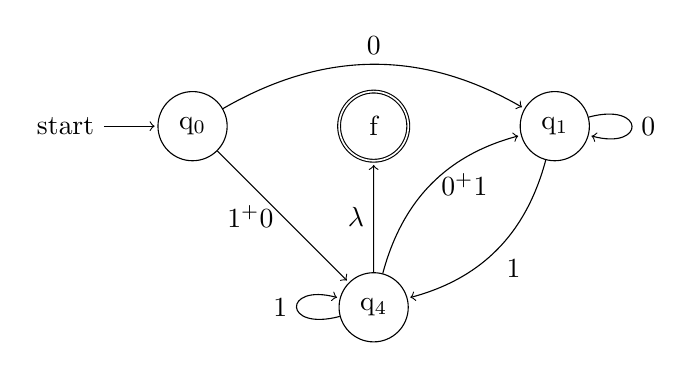
\begin{tikzpicture}[shorten >=1pt, scale=1.5, node distance=2.3cm, on grid, auto][h]
        \node[state, initial] (q0) {$\mathrm{q}_{0}$};
        \node[state, accepting] (a) [right=of q0] {f};
        \node[state] (q1) [right=of a] {$\mathrm{q}_{1}$};
        \node[state, draw=none] (q2) [below of=q1] {};
        \node[state, draw=none] (q3) [below of=q0] {};
        \node[state] (q4) [right=of q3] {$\mathrm{q}_4$};
      
        \path[->]
          (q0) edge[bend left] node {0} (q1)
              (q0) edge node[left] {$1^+ 0$} (q4)
          (q1) edge [loop right] node {0} (q1)
              (q1) edge[bend left] node {1} (q4)
        %   (q2) edge node[right] {1} (q1)
        %       (q2) edge [loop right] node {0} (q2)
        %   (q3) edge [loop left] node {1} (q3)
        %       (q3) edge node[below] {0} (q4)
          (q4) edge [loop left] node {1} (q4)
            %   (q4) edge node[below] {0} (q2)
            (q4) edge node {$\lambda$} (a)
            (q4) edge[bend left] node[right] {$0^+1$} (q1);
      \end{tikzpicture}
\end{minipage}
\hfill
\begin{minipage}[h]{0.48\textwidth}
    \noindent $\bullet$ Step 4: Rip $\mathrm{q}_1$.\\
    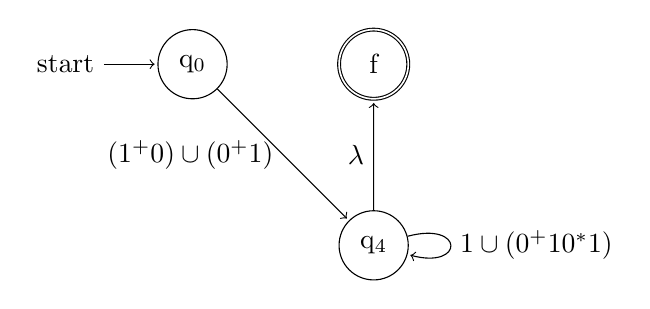
\begin{tikzpicture}[shorten >=1pt, scale=1.5, node distance=2.3cm, on grid, auto][h]
        \node[state, initial] (q0) {$\mathrm{q}_{0}$};
        \node[state, accepting] (a) [right=of q0] {f};
        \node[state, draw=none] (q1) [right=of a] {};
        \node[state, draw=none] (q2) [below of=q1] {};
        \node[state, draw=none] (q3) [below of=q0] {};
        \node[state] (q4) [right=of q3] {$\mathrm{q}_4$};
      
        \path[->]
        %   (q0) edge[bend left] node {0} (q1)
              (q0) edge node[left] {$(1^+ 0) \cup (0^+1)$} (q4)
        %   (q1) edge [loop above] node {0} (q1)
        %       (q1) edge[bend left] node {1} (q4)
        %   (q2) edge node[right] {1} (q1)
        %       (q2) edge [loop right] node {0} (q2)
        %   (q3) edge [loop left] node {1} (q3)
        %       (q3) edge node[below] {0} (q4)
        (q4) edge [loop right] node {$1 \cup (0^+10^*1)$} (q4)
            %   (q4) edge node[below] {0} (q2)
            (q4) edge node {$\lambda$} (a);
            % (q4) edge[bend left] node[right] {$0^+1$} (q1);
      \end{tikzpicture}
\end{minipage}
\newline

\noindent $\bullet$ Step 5: Rip $\mathrm{q}_4$.\\
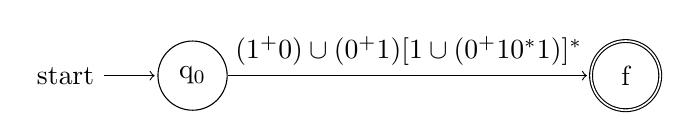
\begin{tikzpicture}[shorten >=1pt, scale=1.5, node distance=5.5cm, on grid, auto][h]
    \node[state, initial] (q0) {$\mathrm{q}_{0}$};
    \node[state, accepting] (a) [right=of q0] {f};
  
    \path[->]
    (q0) edge node[above] {$(1^+0)\cup(0^+1)[1\cup(0^+10^*1)]^*$} (a);
\end{tikzpicture}
\newline
\noindent $\implies$ Hence, the regular expression for the finite automata is: $(1^+0)\cup(0^+1)[1\cup(0^+10^*1)]^*$.
}
\pagebreak

% Cau 2
\qs{Convert the folowing finite automata into equivalent regular expressions}{
$M=\left(Q, \sum, \delta, q_0, F\right) \text { with } \\
Q=\left\{q_0, q_1, q_2, q_3\right\} \\
\sum=\{0,1\} \\
F=\left\{q_3\right\}, \text { and delta is defined by }\\$
\begin{table}[H]
    \centering
    \begin{tabular}{|c|c|c|}
    \hline
    $\delta$ & 0     & 1     \\ \hline
    $q_0$    & $q_2$ & $q_1$ \\ \hline
    $q_1$    & $q_1$ & $q_3$ \\ \hline
    $q_2$    & $q_2$ & $q_1$ \\ \hline
    $q_3$    & $q_3$ & $q_3$ \\ \hline
    \end{tabular}
\end{table}}

\sol{\newline
From the state transition table, we construct the NFA.\\

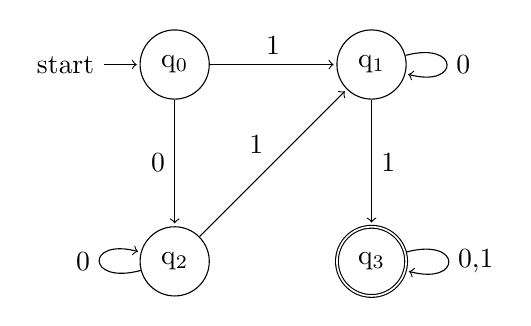
\begin{tikzpicture}[shorten >=1pt, node distance=2.5cm, on grid, auto][h]
  \node[state, initial] (q0) {$\mathrm{q}_{0}$};
  \node[state] (q1) [right=of q0] {$\mathrm{q}_{1}$};
  \node[state] (q2) [below of=q0] {$\mathrm{q}_{2}$};
  \node[state, accepting] (q3) [below of=q1] {$\mathrm{q}_{3}$};

    \path[->]
    (q0) edge node {1} (q1)
        (q0) edge node[left] {0} (q2)
    (q1) edge[loop right] node {0} (q1)
        (q1) edge node {1} (q3)
    (q2) edge[loop left] node {0} (q2)
        (q2) edge node {1} (q1)
    (q3) edge[loop right] node {0,1} (q3);
\end{tikzpicture}
\\
\begin{minipage}[h]{0.48\textwidth}
\noindent $\bullet$ Step 1: Adding new end state.\\
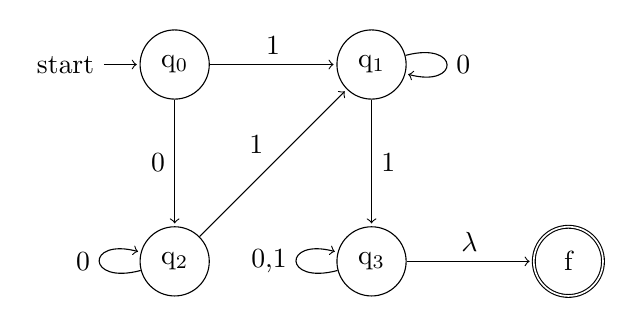
\begin{tikzpicture}[shorten >=1pt, node distance=2.5cm, on grid, auto][h]
    \node[state, initial] (q0) {$\mathrm{q}_{0}$};
    \node[state] (q1) [right=of q0] {$\mathrm{q}_{1}$};
    \node[state] (q2) [below of=q0] {$\mathrm{q}_{2}$};
    \node[state] (q3) [below of=q1] {$\mathrm{q}_{3}$};
    \node[state, accepting] (f) [right=of q3] {f};
  
      \path[->]
      (q0) edge node {1} (q1)
          (q0) edge node[left] {0} (q2)
      (q1) edge[loop right] node {0} (q1)
          (q1) edge node {1} (q3)
      (q2) edge[loop left] node {0} (q2)
          (q2) edge node {1} (q1)
      (q3) edge[loop left] node {0,1} (q3)
        (q3) edge node {$\lambda$} (f);
  \end{tikzpicture}
\end{minipage}
\hfill
\begin{minipage}[h]{0.48\textwidth}
    \noindent $\bullet$ Step 2: Rip $\mathrm{q}_2$.\\
    \begin{tikzpicture}[shorten >=1pt, node distance=3.5cm, on grid, auto][h]
        \node[state, initial] (q0) {$\mathrm{q}_{0}$};
        \node[state] (q1) [right=of q0] {$\mathrm{q}_{1}$};
        % \node[state] (q2) [below of=q0] {$\mathrm{q}_{2}$};
        \node[state] (q3) [below of=q1] {$\mathrm{q}_{3}$};
        \node[state, accepting] (f) [right=of q3] {f};
      
          \path[->]
          (q0) edge node {$1\cup(0^+1)$} (q1)
            %   (q0) edge node[left] {0} (q2)
          (q1) edge[loop right] node {0} (q1)
              (q1) edge node {1} (q3)
        %   (q2) edge[loop left] node {0} (q2)
        %       (q2) edge node {1} (q1)
          (q3) edge[loop left] node {0,1} (q3)
            (q3) edge node {$\lambda$} (f);
      \end{tikzpicture}
\end{minipage}
\begin{minipage}[h]{0.48\textwidth}
    \noindent $\bullet$ Step 3: Rip $\mathrm{q}_3$.\\
    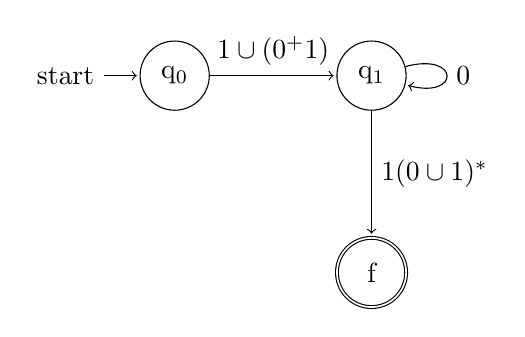
\begin{tikzpicture}[shorten >=1pt, node distance=2.5cm, on grid, auto][h]
        \node[state, initial] (q0) {$\mathrm{q}_{0}$};
        \node[state] (q1) [right=of q0] {$\mathrm{q}_{1}$};
        \node[state, accepting] (f) [below of=q1] {f};
      
        \path[->]
        (q0) edge node {$1\cup(0^+1)$} (q1)
        (q1) edge[loop right] node {0} (q1)
            (q1) edge node {$1(0 \cup 1)^*$} (f);
      \end{tikzpicture}
\end{minipage}
\hfill
\begin{minipage}[h]{0.48\textwidth}
    \noindent $\bullet$ Step 4: Rip $\mathrm{q}_1$.\\
    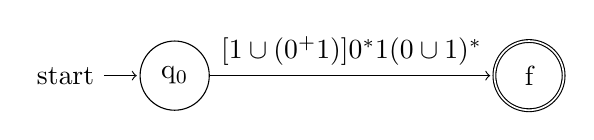
\begin{tikzpicture}[shorten >=1pt, node distance=4.5cm, on grid, auto][h]
        \node[state, initial] (q0) {$\mathrm{q}_0$};
        \node[state, accepting] (f) [right=of q0] {f};

        \path[->]
        (q0) edge node {$[1 \cup (0^+1)] 0^*1(0\cup1)^*$} (f);
    \end{tikzpicture}
    
\end{minipage}
\newline

\noindent $\implies$ Hence, the regular expression for the finite automata is: $[1 \cup (0^+1)] 0^*1(0\cup1)^*$.
}
\pagebreak

% Cau 3
\qs{Convert the folowing finite automata into equivalent regular expressions}{
$
M=\left(Q, \sum, \delta, q_0, F\right) \text { with } \\
Q=\left\{q_0, q_1, q_2, q_3, q_4, q_5, q_6, q_7\right\} \\
\sum=\{0,1\} \\
F=\left\{q_3\right\}, \text { and } \delta \text { is defined by }$
\begin{table}[H]
    \centering
    \begin{tabular}[h]{|c|c|c|}
        \hline $\delta$ & 0 & 1 \\
        \hline $q_0$ & $q_1$ & $q_0$ \\
        \hline $q_1$ & $q_0$ & $q_2$ \\
        \hline $q_2$ & $q_3$ & $q_1$ \\
        \hline $q_3$ & $q_3$ & $q_0$ \\
        \hline $q_4$ & $q_3$ & $q_5$ \\
        \hline $q_5$ & $q_6$ & $q_4$ \\
        \hline $q_6$ & $q_5$ & $q_6$ \\
        \hline $q_7$ & $q_6$ & $q_3$ \\
        \hline
        \end{tabular} 
\end{table}}

\sol{\newline
From the above information, let us construct the corresponding NFA.\\
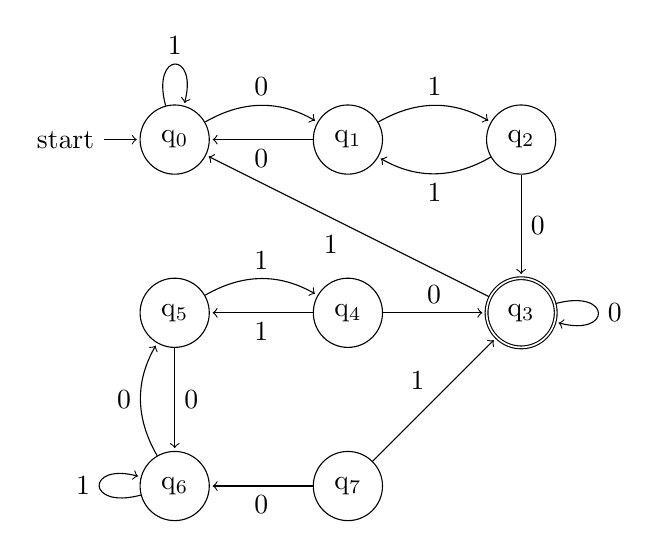
\begin{tikzpicture}[shorten >=1pt, node distance=2.2cm, on grid, auto][h]
    \node[state, initial] (q0) {$\mathrm{q}_0$};
    \node[state] (q1) [right=of q0] {$\mathrm{q}_1$};
    \node[state] (q2) [right=of q1] {$\mathrm{q}_2$};
    \node[state, accepting] (q3) [below of=q2] {$\mathrm{q}_3$};
    \node[state] (q4) [below of=q1] {$\mathrm{q}_4$};
    \node[state] (q5) [below of=q0] {$\mathrm{q}_5$};
    \node[state] (q6) [below of=q5] {$\mathrm{q}_6$};
    \node[state] (q7) [right=of q6] {$\mathrm{q}_7$};

    \path[->]
    (q0) edge[bend left] node {0} (q1)
        (q0) edge[loop above] node {1} (q0)
    (q1) edge node {0} (q0)
        (q1) edge[bend left] node {1} (q2)
    (q2) edge node {0} (q3)
        (q2) edge[bend left] node {1} (q1)
    (q3) edge[loop right] node {0} (q3)
        (q3) edge node {1} (q0)
    (q4) edge node {0} (q3)
        (q4) edge node {1} (q5)
    (q5) edge[bend left] node {1} (q4)
        (q5) edge node {0} (q6)
    (q6) edge[bend left] node {0} (q5)
        (q6) edge[loop left] node {1} (q6)
    (q7) edge node {0} (q6)
        (q7) edge node {1} (q3);
\end{tikzpicture}
\newline
Let us insert new ending state and starting state.\\
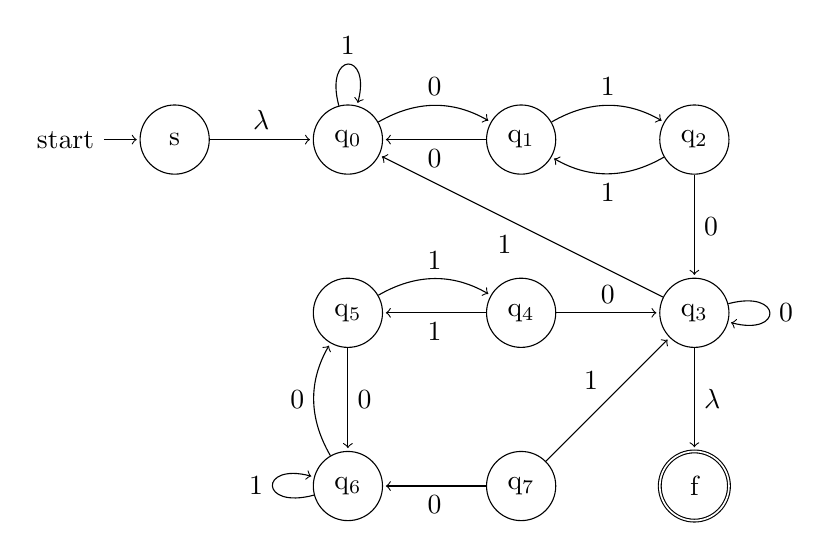
\begin{tikzpicture}[shorten >=1pt, node distance=2.2cm, on grid, auto][h]
    \node[state, initial] (s) {s};
    \node[state] (q0) [right=of s] {$\mathrm{q}_0$};
    \node[state] (q1) [right=of q0] {$\mathrm{q}_1$};
    \node[state] (q2) [right=of q1] {$\mathrm{q}_2$};
    \node[state] (q3) [below of=q2] {$\mathrm{q}_3$};
    \node[state] (q4) [below of=q1] {$\mathrm{q}_4$};
    \node[state] (q5) [below of=q0] {$\mathrm{q}_5$};
    \node[state] (q6) [below of=q5] {$\mathrm{q}_6$};
    \node[state] (q7) [right=of q6] {$\mathrm{q}_7$};
    \node[state, accepting] (f) [below of=q3] {f};

    \path[->]
    (s) edge node {$\lambda$} (q0)
    (q0) edge[bend left] node {0} (q1)
        (q0) edge[loop above] node {1} (q0)
    (q1) edge node {0} (q0)
        (q1) edge[bend left] node {1} (q2)
    (q2) edge node {0} (q3)
        (q2) edge[bend left] node {1} (q1)
    (q3) edge[loop right] node {0} (q3)
        (q3) edge node {1} (q0)
        (q3) edge node {$\lambda$} (f)
    (q4) edge node {0} (q3)
        (q4) edge node {1} (q5)
    (q5) edge[bend left] node {1} (q4)
        (q5) edge node {0} (q6)
    (q6) edge[bend left] node {0} (q5)
        (q6) edge[loop left] node {1} (q6)
    (q7) edge node {0} (q6)
        (q7) edge node {1} (q3);
\end{tikzpicture}
\pagebreak

\noindent $\bullet$ Since $\mathrm{q}_7$ has no path leading to it, we can remove it without affecting the automaton.\\
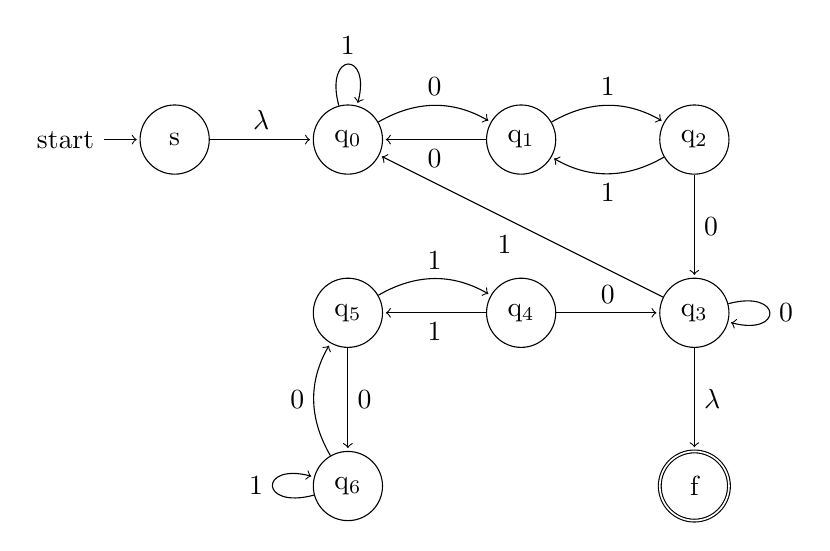
\begin{tikzpicture}[shorten >=1pt, node distance=2.2cm, on grid, auto][h]
    \node[state, initial] (s) {s};
    \node[state] (q0) [right=of s] {$\mathrm{q}_0$};
    \node[state] (q1) [right=of q0] {$\mathrm{q}_1$};
    \node[state] (q2) [right=of q1] {$\mathrm{q}_2$};
    \node[state] (q3) [below of=q2] {$\mathrm{q}_3$};
    \node[state] (q4) [below of=q1] {$\mathrm{q}_4$};
    \node[state] (q5) [below of=q0] {$\mathrm{q}_5$};
    \node[state] (q6) [below of=q5] {$\mathrm{q}_6$};
    \node[state, accepting] (f) [below of=q3] {f};

    \path[->]
    (s) edge node {$\lambda$} (q0)
    (q0) edge[bend left] node {0} (q1)
        (q0) edge[loop above] node {1} (q0)
    (q1) edge node {0} (q0)
        (q1) edge[bend left] node {1} (q2)
    (q2) edge node {0} (q3)
        (q2) edge[bend left] node {1} (q1)
    (q3) edge[loop right] node {0} (q3)
        (q3) edge node {1} (q0)
        (q3) edge node {$\lambda$} (f)
    (q4) edge node {0} (q3)
        (q4) edge node {1} (q5)
    (q5) edge[bend left] node {1} (q4)
        (q5) edge node {0} (q6)
    (q6) edge[bend left] node {0} (q5)
        (q6) edge[loop left] node {1} (q6);
\end{tikzpicture}
\newline
\begin{minipage}{0.48\textwidth}
    \noindent $\bullet$ Step 1: Rip out $\mathrm{q}_6$.\\
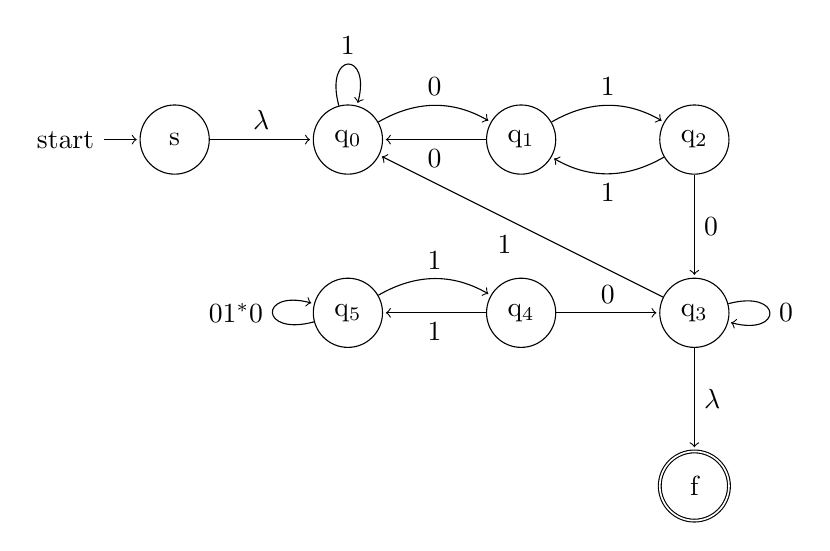
\begin{tikzpicture}[shorten >=1pt, node distance=2.2cm, on grid, auto][h]
    \node[state, initial] (s) {s};
    \node[state] (q0) [right=of s] {$\mathrm{q}_0$};
    \node[state] (q1) [right=of q0] {$\mathrm{q}_1$};
    \node[state] (q2) [right=of q1] {$\mathrm{q}_2$};
    \node[state] (q3) [below of=q2] {$\mathrm{q}_3$};
    \node[state] (q4) [below of=q1] {$\mathrm{q}_4$};
    \node[state] (q5) [below of=q0] {$\mathrm{q}_5$};
    \node[state, accepting] (f) [below of=q3] {f};

    \path[->]
    (s) edge node {$\lambda$} (q0)
    (q0) edge[bend left] node {0} (q1)
        (q0) edge[loop above] node {1} (q0)
    (q1) edge node {0} (q0)
        (q1) edge[bend left] node {1} (q2)
    (q2) edge node {0} (q3)
        (q2) edge[bend left] node {1} (q1)
    (q3) edge[loop right] node {0} (q3)
        (q3) edge node {1} (q0)
        (q3) edge node {$\lambda$} (f)
    (q4) edge node {0} (q3)
        (q4) edge node {1} (q5)
    (q5) edge[bend left] node {1} (q4)
        (q5) edge[loop left] node {$01^*0$} (q5);
\end{tikzpicture}
\end{minipage}
\hfill
\begin{minipage}{0.48\textwidth}
    \noindent $\bullet$ Step 2: Rip out $\mathrm{q}_5$.\\
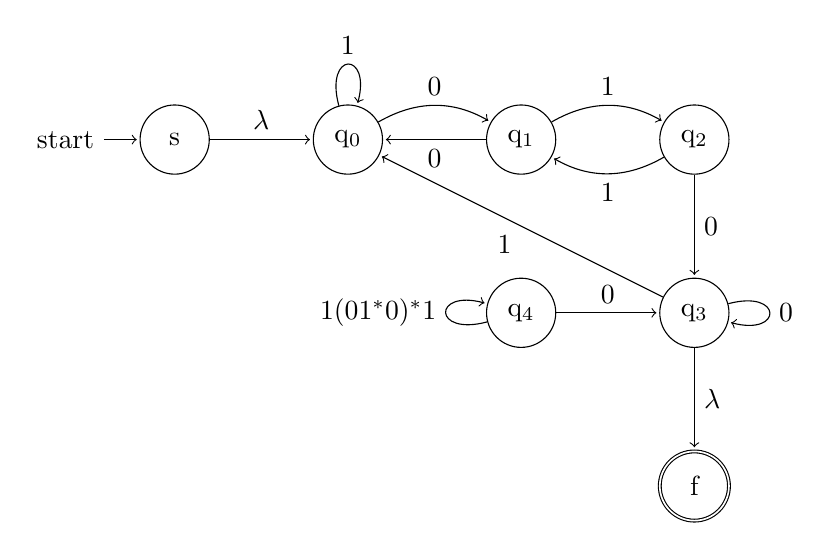
\begin{tikzpicture}[shorten >=1pt, node distance=2.2cm, on grid, auto][h]
    \node[state, initial] (s) {s};
    \node[state] (q0) [right=of s] {$\mathrm{q}_0$};
    \node[state] (q1) [right=of q0] {$\mathrm{q}_1$};
    \node[state] (q2) [right=of q1] {$\mathrm{q}_2$};
    \node[state] (q3) [below of=q2] {$\mathrm{q}_3$};
    \node[state] (q4) [below of=q1] {$\mathrm{q}_4$};
    \node[state, accepting] (f) [below of=q3] {f};

    \path[->]
    (s) edge node {$\lambda$} (q0)
    (q0) edge[bend left] node {0} (q1)
        (q0) edge[loop above] node {1} (q0)
    (q1) edge node {0} (q0)
        (q1) edge[bend left] node {1} (q2)
    (q2) edge node {0} (q3)
        (q2) edge[bend left] node {1} (q1)
    (q3) edge[loop right] node {0} (q3)
        (q3) edge node {1} (q0)
        (q3) edge node {$\lambda$} (f)
    (q4) edge node {0} (q3)
        (q4) edge[loop left] node {$1(01^*0)^*1$} (q4);
\end{tikzpicture}
\end{minipage}
\newline
\noindent $\bullet$ Since $\mathrm{q}_4$ has no path leading to it, we can remove it without affecting the automaton.\\
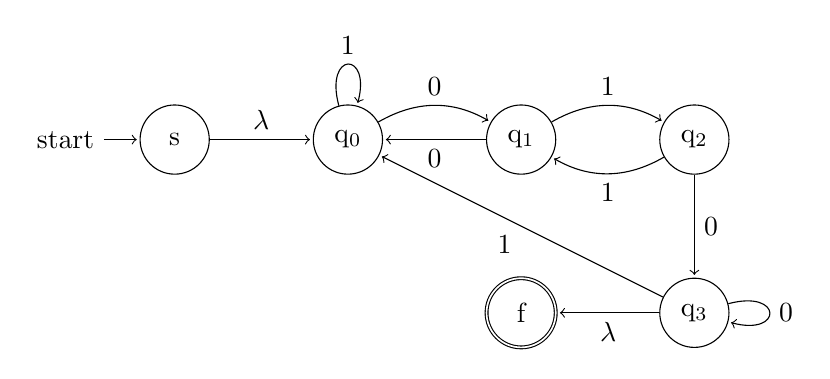
\begin{tikzpicture}[shorten >=1pt, node distance=2.2cm, on grid, auto][h]
    \node[state, initial] (s) {s};
    \node[state] (q0) [right=of s] {$\mathrm{q}_0$};
    \node[state] (q1) [right=of q0] {$\mathrm{q}_1$};
    \node[state] (q2) [right=of q1] {$\mathrm{q}_2$};
    \node[state] (q3) [below of=q2] {$\mathrm{q}_3$};
    \node[state, accepting] (f) [left=of q3] {f};

    \path[->]
    (s) edge node {$\lambda$} (q0)
    (q0) edge[bend left] node {0} (q1)
        (q0) edge[loop above] node {1} (q0)
    (q1) edge node {0} (q0)
        (q1) edge[bend left] node {1} (q2)
    (q2) edge node {0} (q3)
        (q2) edge[bend left] node {1} (q1)
    (q3) edge[loop right] node {0} (q3)
        (q3) edge node {1} (q0)
        (q3) edge node {$\lambda$} (f);
\end{tikzpicture}
\newline
\begin{minipage}{0.48\textwidth}
    \noindent $\bullet$ Step 3: Rip $\mathrm{q}_3$.\\
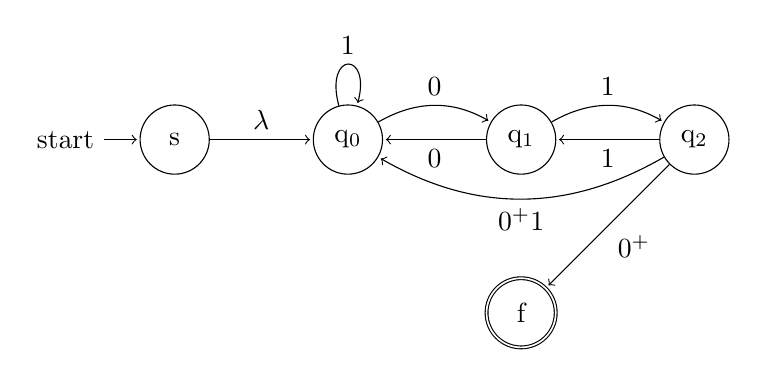
\begin{tikzpicture}[shorten >=1pt, node distance=2.2cm, on grid, auto][h]
    \node[state, initial] (s) {s};
    \node[state] (q0) [right=of s] {$\mathrm{q}_0$};
    \node[state] (q1) [right=of q0] {$\mathrm{q}_1$};
    \node[state] (q2) [right=of q1] {$\mathrm{q}_2$};
    \node[state, accepting] (f) [below of=q1] {f};

    \path[->]
    (s) edge node {$\lambda$} (q0)
    (q0) edge[bend left] node {0} (q1)
        (q0) edge[loop above] node {1} (q0)
    (q1) edge node {0} (q0)
        (q1) edge[bend left] node {1} (q2)
    (q2) edge[bend left] node {$0^+1$} (q0)
        (q2) edge node {$0^+$} (f)
        (q2) edge node {1} (q1);
\end{tikzpicture}
\end{minipage}
\hfill
\begin{minipage}{0.48\textwidth}
    \noindent $\bullet$ Step 4: Rip $\mathrm{q}_0$.\\
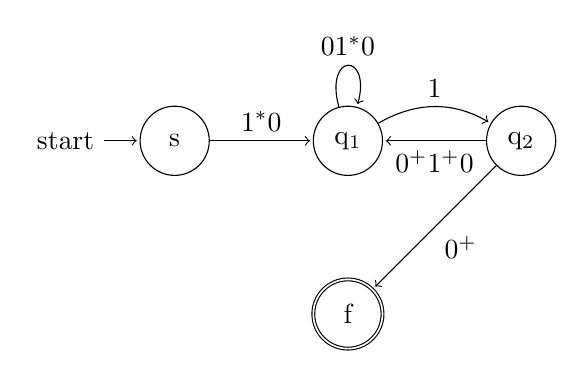
\begin{tikzpicture}[shorten >=1pt, node distance=2.2cm, on grid, auto][h]
    \node[state, initial] (s) {s};
    \node[state] (q1) [right=of s] {$\mathrm{q}_1$};
    \node[state] (q2) [right=of q1] {$\mathrm{q}_2$};
    \node[state, accepting] (f) [below of=q1] {f};

    \path[->]
    % (s) edge node {$\lambda$} (q0)
        (s) edge node {$1^*0$} (q1)
    % (q0) edge[bend left] node {0} (q1)
    %     (q0) edge[loop above] node {1} (q0)
    (q1) edge[loop above] node {$01^*0$} (q1)
        (q1) edge[bend left] node {1} (q2)
    % (q2) edge[bend left] node {$0^+1$} (q0)
        (q2) edge node {$0^+$} (f)
        (q2) edge node {$0^+1^+0$} (q1);
\end{tikzpicture}
\end{minipage}
\pagebreak
\begin{minipage}{0.48\textwidth}
    \noindent $\bullet$ Step 5: Rip $\mathrm{q}_2$.\\
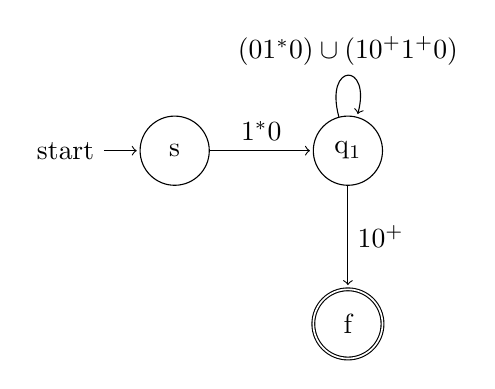
\begin{tikzpicture}[shorten >=1pt, node distance=2.2cm, on grid, auto][h]
    \node[state, initial] (s) {s};
    \node[state] (q1) [right=of s] {$\mathrm{q}_1$};
    \node[state, accepting] (f) [below of=q1] {f};

    \path[->]
    (s) edge node {$1^*0$} (q1)
    (q1) edge[loop above] node {$(01^*0)\cup(10^+1^+0)$} (q1)
        (q1) edge node {$10^+$} (f);
\end{tikzpicture}
\end{minipage}
\hfill
\begin{minipage}{0.48\textwidth}
    \noindent $\bullet$ Step 6: Rip $\mathrm{q}_1$.\\
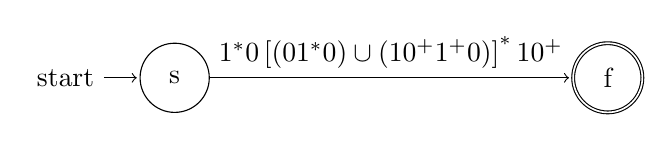
\begin{tikzpicture}[shorten >=1pt, node distance=5.5cm, on grid, auto][h]
    \node[state, initial] (s) {s};
    \node[state, accepting] (f) [right=of s] {f};

    \path[->]
    (s) edge node {$1^*0\left[(01^*0)\cup(10^+1^+0)\right]^*10^+$} (f);
\end{tikzpicture}
\end{minipage}
% \noindent $\implies$ Hence, the regular expression for the finite automata is: $1^*0\left[(01^*0)\cup(10^+1^+0)\right]^*10^+$.
}
\end{document}
